% !TeX spellcheck = cs_CZ
\begin{mdframed}[style=mdexam]
  \begin{example}\label{teo:exam092}
    Je dán trojúhelník s vrcholy \(A[0, 0]\), \(B[4, 0]\), \(C[1, 3]\). Mezi všemi obdélníky
    vepsanými danému trojúhelníku, se stranou („základnou“) \(z\) ve straně \(c\) (označení viz obr.
    \ref{mai:fig062}), máme najít ten, který má maximální obsah.

    {\centering
      \captionsetup{type=figure}
      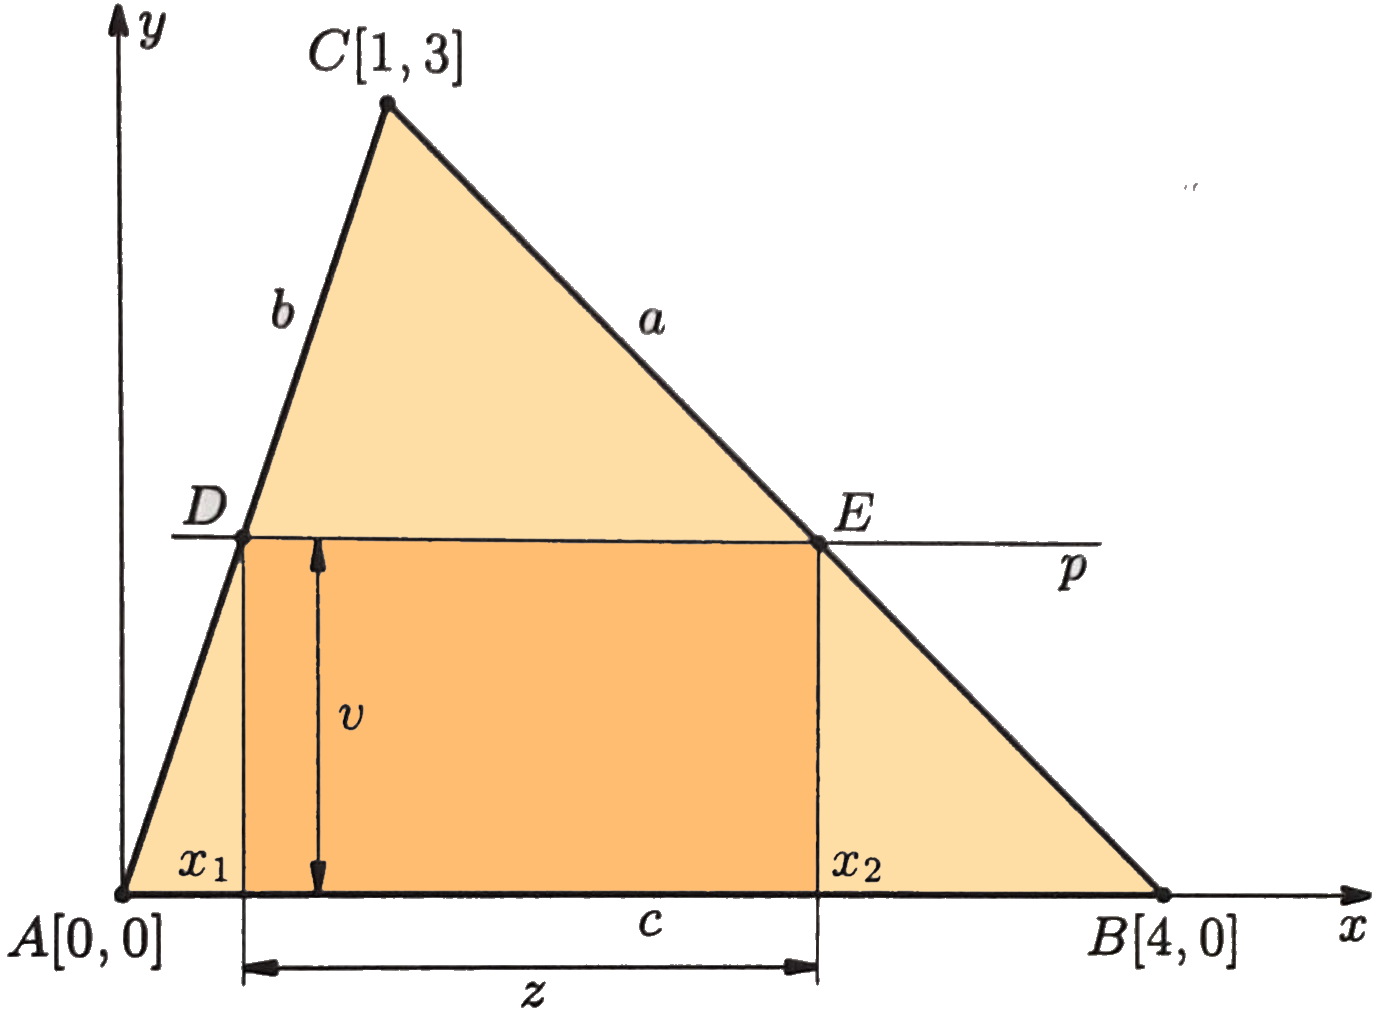
\includegraphics[width=0.7\linewidth]{mai_fig062.png} 
      \captionof{figure}{K příkladu \ref{teo:exam092}. Kredit: \cite[s.~46]{rektorys2011}}
      \label{mai:fig062}
    \par}
    
    Napišme nejprve rovnice stran \(a\), \(b\). Strana \(b\) (přesněji: přímka obsahující stranu
    \(b\)) má zřejmě rovnici
    \begin{equation*}
      y = 3x
    \end{equation*}
    Přímka, v níž leží strana \(a\), má směrnici
    \begin{equation*}
      k = \dfrac{3-0}{1-4} = -1,
    \end{equation*}
    a tedy podle rovnice \(y-y_0 = k(x-x_0)\) dostáváme 
    \begin{equation*}
      y - 0 = -1\cdot(x - 4) \quad\Rightarrow\quad y = -x + 4.  
    \end{equation*}
    Pro obsah \(S\) vepsaného obdélníka platí podle označení v obr. \ref{mai:fig062} 
    \begin{equation*}
      S = zv.
    \end{equation*}
    Za proměnnou zde bude výhodné volit „výšku“ \(v\). „Základnu“ \(z\) pak vypočteme (viz obr.
    \ref{mai:fig062}) jako rozdíl
    \begin{equation}\label{mai:eq087}
      z = x_2 - x_1,
    \end{equation}
    kde \(x_1\), resp. \(x_2\) je souřadnice \(x\) průsečíku přímky \(y = v\) (přímka \(p\) na obr.
    \ref{mai:fig062}) se stranou \(b\), resp. \(a\). Rovnice těchto stran jsou dány vztahy \(y =
    3x\) a \(y = -x + 4\). Dosadíme-li podle \(y = v\rightarrow\)  \(v\) za \(y\) do těchto rovnic,
    dostaneme právě \(x_1\) a \(x_2\). Bude
    \begin{equation*}
      v = 3x_1, \qquad\qquad v = -x_2 + 4,
    \end{equation*}
    odkud (při zvoleném \(v\)) plyne
    \begin{equation*}
      x_1 = \dfrac{v}{3}, \qquad\qquad  x_2 = 4 - v 
    \end{equation*}
    a podle \ref{mai:eq087}
    \begin{equation*}
      z = x_2 - x_1 =  4 - \dfrac{4}{3}v
    \end{equation*}
    a konečně pro obsah vepsaného obdélníku dostáváme jednoduchou rovnici
    \begin{equation}\label{mai:eq088}
      S = zv = \left(4 - \dfrac{4}{3}v\right)v = 4v - \dfrac{4}{3}v^2.
    \end{equation} 
    Tím je obsah \(S\) obdélníka daný jako funkce zvolené výšky \(v\). Zvolíme-li například \(v=1\),
    bude obsah \(S\) obdélníka z obr. \ref{mai:fig062} roven číslu \(4\cdot1 -
    \frac{4}{3}\cdot1^2\). 
    
    Budeme hledat (absolutní) maximum funkce (\ref{mai:eq088}) na intervalu \(\langle0,3\rangle\)
    (neboť nemůžeme zvolit \(v\) větší než 3). Ale pro \(v=0\) a \(v=3\) je \(S=0\) a všude jinde je
    \(S > 0\), takže budeme hledat lokální maximum funkce (\ref{mai:eq088}) na otevřeném intervalu
    \((0,3)\). Derivováním (\ref{mai:eq088}) podle proměnné \(v\) však máme
    \begin{equation*}
      S' = 4 - \dfrac{8}{3}v, \qquad\qquad S'' = -\dfrac{8}{3}.
    \end{equation*}
    Položíme-li nyní pravou stranu rovnu nule, dostaneme 
    \begin{equation*}
      4 - \dfrac{8}{3}v = 0 \quad\Rightarrow\quad v = \dfrac{12}{8} = \dfrac{3}{2}.
    \end{equation*}
    Přitom podle druhé derivace obsahu je všude, a tedy i v bodě \(frac{3}{2}\), je
    \(S''=-\frac{8}{3}<0\) takže v bodě \(v = \frac{2}{3}\) je ostré lokální maximum. Zároveň pro
    \(v=\frac{3}{2}\) bude
    \begin{equation*}
      z = 4 - \dfrac{4}{3}\cdot\dfrac{3}{2} = 2.
    \end{equation*}
    Hledaný obdélník maximálního obsahu bude mít rozměry: \(z = 2\), \(v = \frac{3}{2}\), a tedy
    obsah \(S = 3\).    
  \end{example}
\end{mdframed}


